%%=============================================================================
%% resultaten vergelijkend onderzoek
%%=============================================================================

\chapter{Resultaten vergelijkend onderzoek}
\label{ch:Resultaten vergelijkend onderzoek}
Wie in detail wilt bekijken hoe de resultaten zijn bekomen, kan meer informatie vinden bij \ref{appendix:stappenplan analyse}.

\section{Vergelijking van de assistenten in spraakkwaliteit}
\label{s:Vergelijking van de assistenten in spraakkwaliteit}

\subsection{Vergelijking van de assistenten per eigenschap}
\label{ss:Vergelijking van de assistenten per eigenschap}

\begin{figure}[h]
    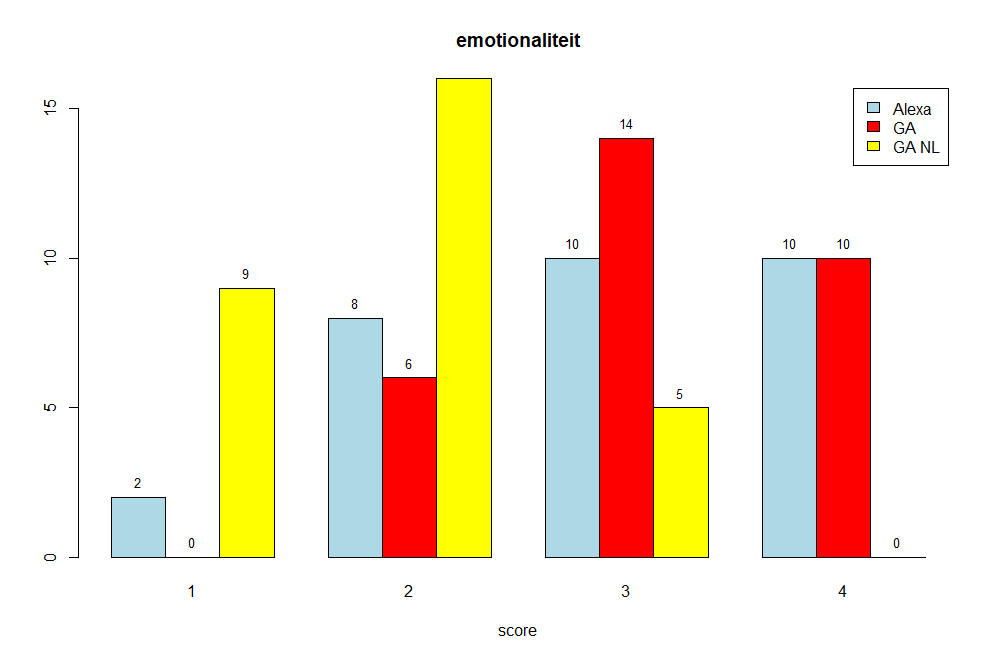
\includegraphics[width=0.9\linewidth]{../onderzoek/onderzoeksresultaten/vergelijking_assistenten_per_eigenschap/barplot/barplot_score_emotionaliteit}
    \caption{De score die de deelnemers hebben gegeven op de emotionaliteit van de assistenten}
    \label{fig:barplot-emotionaliteit}
\end{figure}

\begin{figure}[h]
    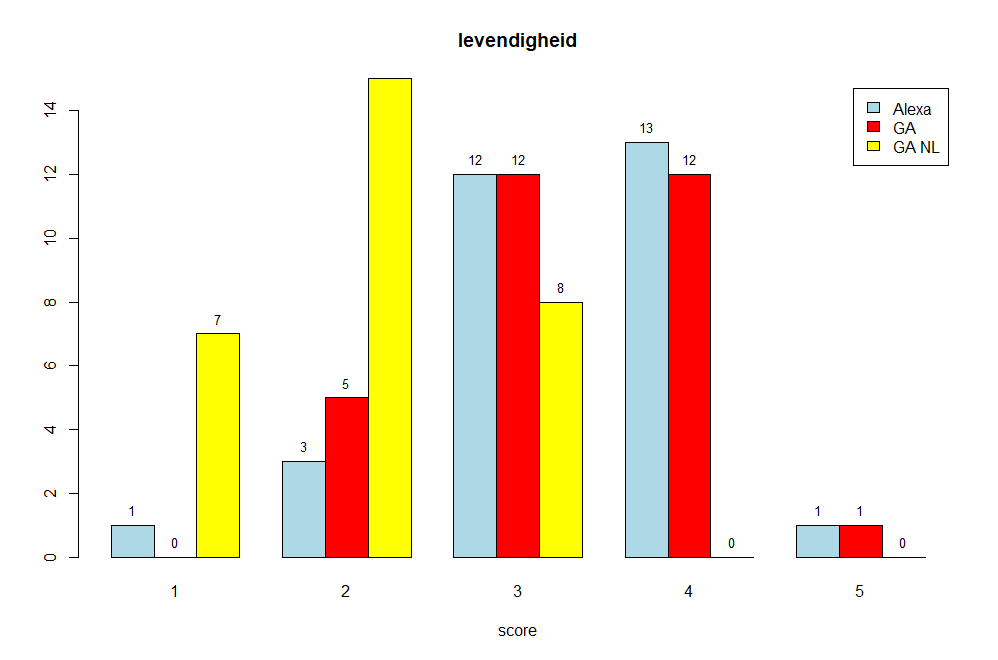
\includegraphics[width=0.9\linewidth]{../onderzoek/onderzoeksresultaten/vergelijking_assistenten_per_eigenschap/barplot/barplot_score_levendigheid}
    \caption{De score die de deelnemers hebben gegeven op de levendigheid van de assistenten}
    \label{fig:barplot-levendigheid}
\end{figure}

\begin{figure}[h]
    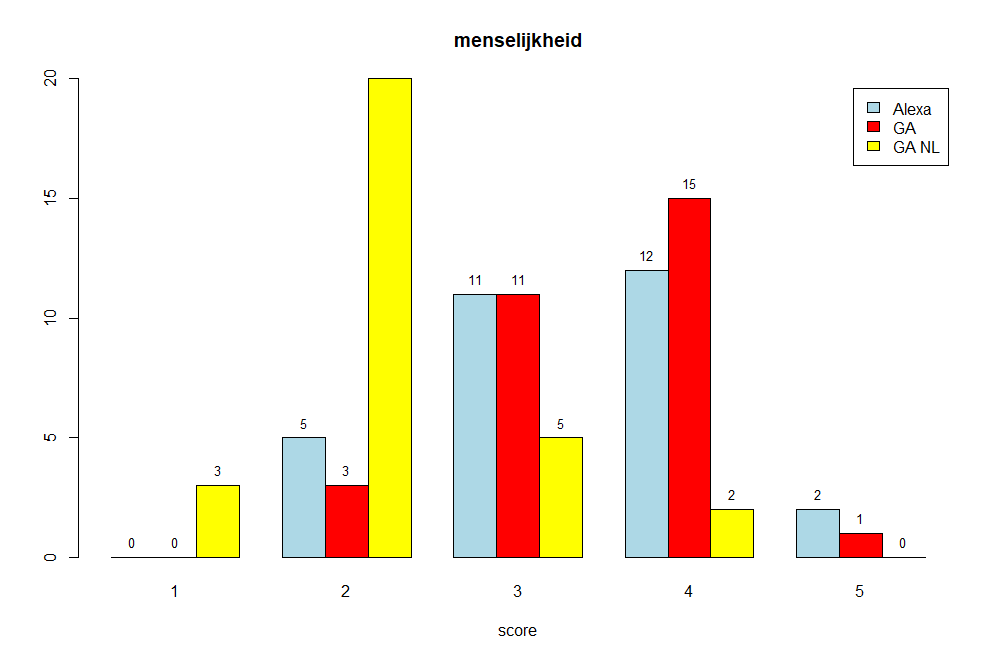
\includegraphics[width=0.9\linewidth]{../onderzoek/onderzoeksresultaten/vergelijking_assistenten_per_eigenschap/barplot/barplot_score_menselijkheid}
    \caption{De score die de deelnemers hebben gegeven op de menselijkheid van de assistenten}
    \label{fig:barplot-menselijkheid}
\end{figure}

\begin{figure}[h]
    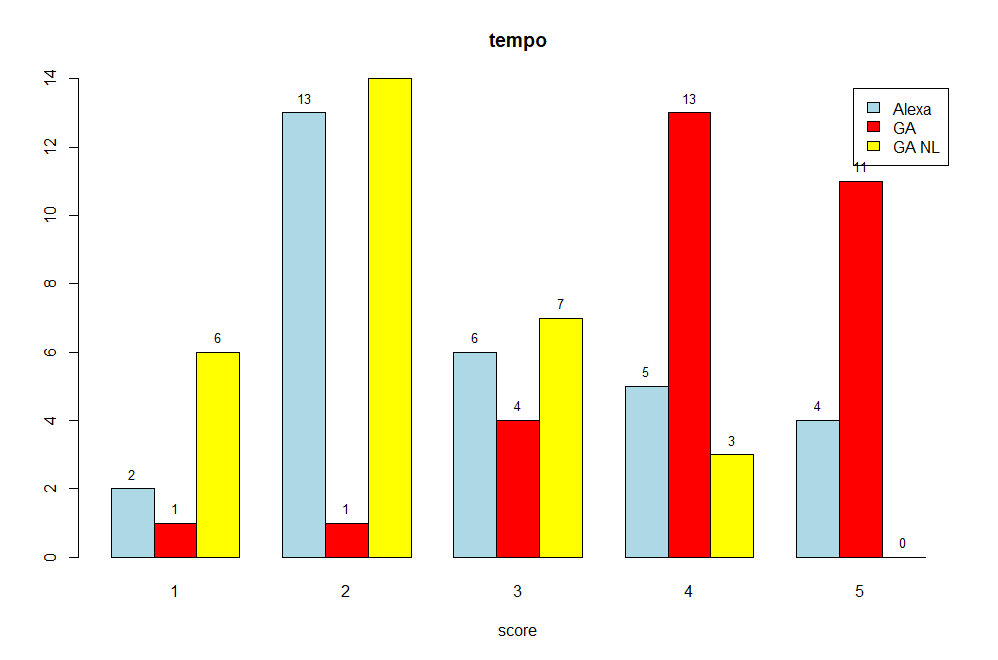
\includegraphics[width=0.9\linewidth]{../onderzoek/onderzoeksresultaten/vergelijking_assistenten_per_eigenschap/barplot/barplot_score_tempo}
    \caption{De score die de deelnemers hebben gegeven op het tempo van de assistenten}
    \label{fig:barplot-tempo}
\end{figure}

\begin{figure}[h]
    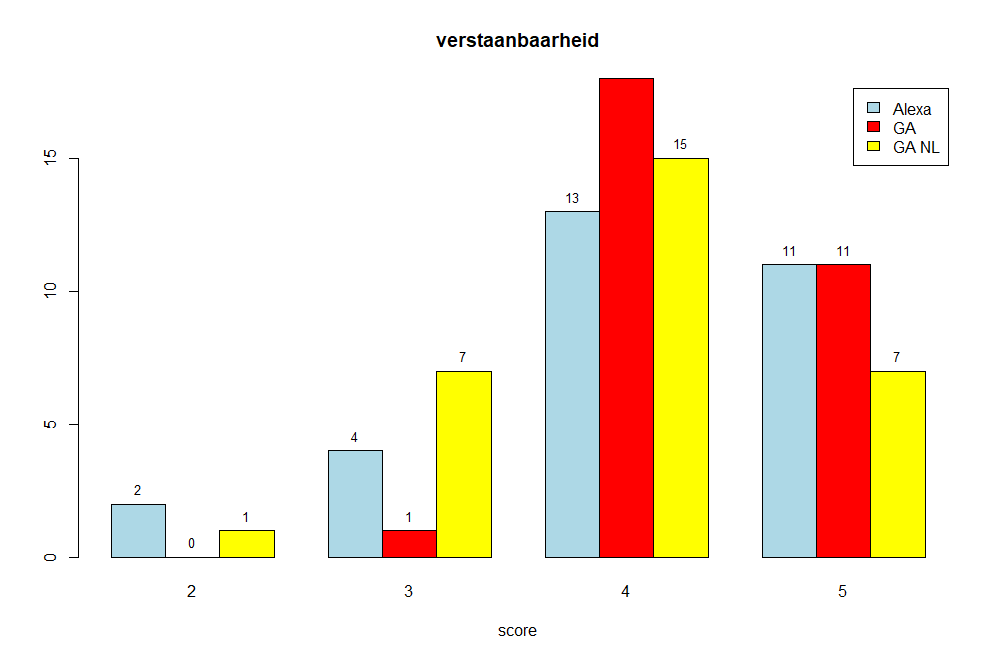
\includegraphics[width=0.9\linewidth]{../onderzoek/onderzoeksresultaten/vergelijking_assistenten_per_eigenschap/barplot/barplot_score_verstaanbaarheid}
    \caption{De score die de deelnemers hebben gegeven op de verstaanbaarheid van de assistenten}
    \label{fig:barplot-verstaanbaarheid}
\end{figure}

\begin{figure}[h]
    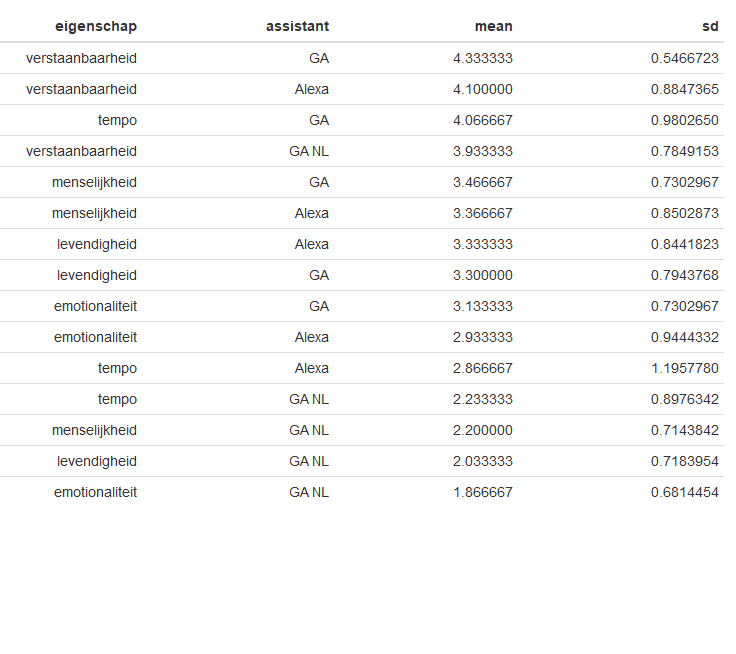
\includegraphics[width=0.9\linewidth]{../onderzoek/onderzoeksresultaten/vergelijking_assistenten_per_eigenschap/table_mean_sd_scores}
    \caption{De gemiddelde score en standaardafwijking van alle assistenten hun eigenschappen gesorteerd van hoog naar laag.}
    \label{fig:table-mean-sd-scores}
\end{figure}

\subsection{Vergelijking van de eigenschappen per assistent}
--Hier boxplots--

De resultaten van de uitgevoerde t-testen zijn te vinden onder de map onderzoek/onderzoeksresultaten in de repository beschreven in \ref{s:verwijzing naar repository}.

De p-waarde ligt bij elke test duidelijk onder het significantieniveau van 0.05 dus kunnen we de nulhypothese verwerpen. De volgende stellingen zijn statistisch verantwoord.
\begin{itemize}
    \item Alexa scoort significant hoger op emotionaliteit dan GA NL.
    \item GA scoort significant hoger op emotionaliteit dan GA NL.
    \item Alexa scoort hoger op levendigheid dan GA NL.
    \item GA scoort hoger op levendigheid dan GA NL.
    \item Alexa scoort hoger op menselijkheid dan GA NL.
    \item GA scoort hoger op menselijkheid dan GA NL.
    \item GA scoort hoger op tempo dan Alexa.
    \item Alexa scoort hoger op tempo dan GA NL.
    \item GA scoort hoger op verstaanbaarheid dan GA NL.
\end{itemize}

\section{Vergelijking van de assistenten in spraakherkenning}
\subsection{Een moeilijk te voeren onderzoek}
Uitleg over hoe moeilijk het was om dit onderzoek correct te voeren ondanks de genomen maatregelen beschreven in de methodologie.

Een eerste bemerking bij het onderzoek is dat elke fout gelijk meetelt. Stel dat twee assistenten de uitspraak 'help me with a burn' omvormen naar tekst. De ene assistent begrijpt de vraag als 'help us for a burn' en de andere als 'tell me with a good'. Alhoewel het gevoel zegt dat de eerste assistent de vraag beter heeft begrepen dan de tweede hebben ze toch allebei evenveel fouten gemaakt. de eerste assistent mist de woorden 'me' en 'with', terwijl de tweede assistent de woorden 'help' en 'burn' mist. Om de correctheid van een gevormde zin beter te interpreteren zou aan elk woord een soort van hoofdzakelijkheid voor het begrijpen van de zin moeten toegekend worden. Er bestaan echter geen vaste regels om dit aan woorden toe te wijzen.

Ondanks dat er verschillende maatregelen zijn genomen om ervoor te zorgen dat elke assistent identiek dezelfde vraag krijgt, is deze opzet toch niet helemaal geslaagd. Alexa neemt elke conversatie op en bewaart ze in uw geschiedenis. Door enkele conversaties van tijdens het onderzoek te beluisteren is er opgemerkt dat hier en daar gekraak aanwezig is. Het gekraak was tijdens het onderzoek niet hoorbaar, waardoor de oorzaak waarschijnlijk bij de microfoon van de smartphone ligt. Het onderzoek is niet correct gevoerd omdat de sterkte van het gekraak kan variëren en mogelijks invloed heeft op de prestaties van de Speech-To-Text-functie van een assistent.

